\begin{surferPage}{An $A_4^{++}$ Singularity}
  As we have seen, the $A_4^{+-}$ singularity looks similar to the $A_2^{+-}$
    singularity.
    Analogously, the $A_4^{++}$ and the $A_2^{++}$ singularity look almost
    identically.  
    The following pictures show the surfaces
    $A_2^{++}$, $A_4^{++}$,$A_2^{+-}$, $A_4^{+-}$:
    \begin{center}
      \vspace*{-0.2cm}
      \begin{tabular}{@{}c@{\ }c@{\ }c@{\ }c@{}}
        \begin{tabular}{@{}c@{}}
          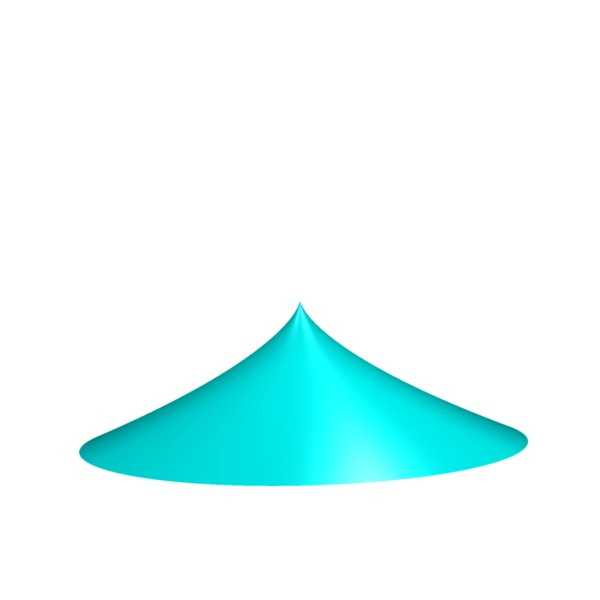
\includegraphics[width=1.2cm]{../../common/images/A2pp}
        \end{tabular}
        &
        \begin{tabular}{@{}c@{}}
          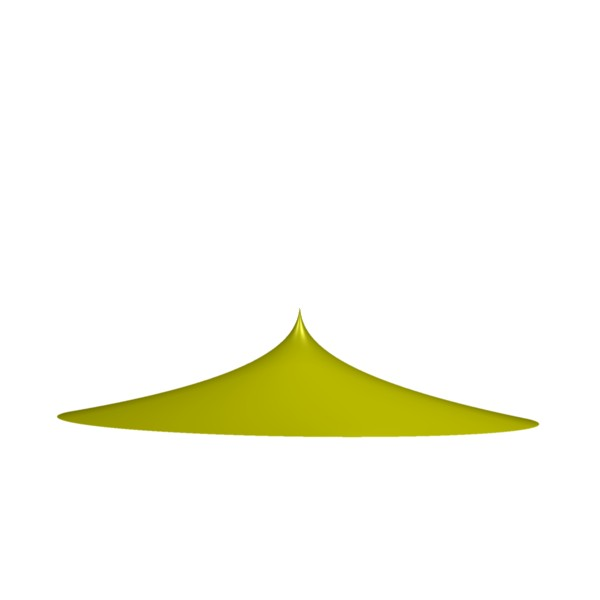
\includegraphics[width=1.2cm]{../../common/images/A4pp}
        \end{tabular}
        &
        \begin{tabular}{@{}c@{}}
          
\includegraphics[width=1.2cm]{../../common/images/A2pm}
        \end{tabular}
        &
        \begin{tabular}{@{}c@{}}
          
\includegraphics[width=1.2cm]{../../common/images/A4pm}
        \end{tabular}
      \end{tabular}
    \end{center}
    \vspace*{-0.2cm}
    One may obseve that the $A_4$ singularities approach the singular point
    more steeply.

    As in the case of the $A_4^{+-}$ singularity, we obtain a significant
    difference to the $A_2$ singularity only by trying to deform the
    singularity into many double cones or a surface with many holes:
    The $A_2^{++}$ singularity can only be deformed into one double cone, the
    $A_4^{++}$ singularity into two double cones:
%    \dontshow{
    % 
    \begin{center}
      \vspace*{-0.2cm}
      \begin{tabular}{@{}c@{\quad}c@{\quad}c@{}}
        \begin{tabular}{@{}c@{}}
          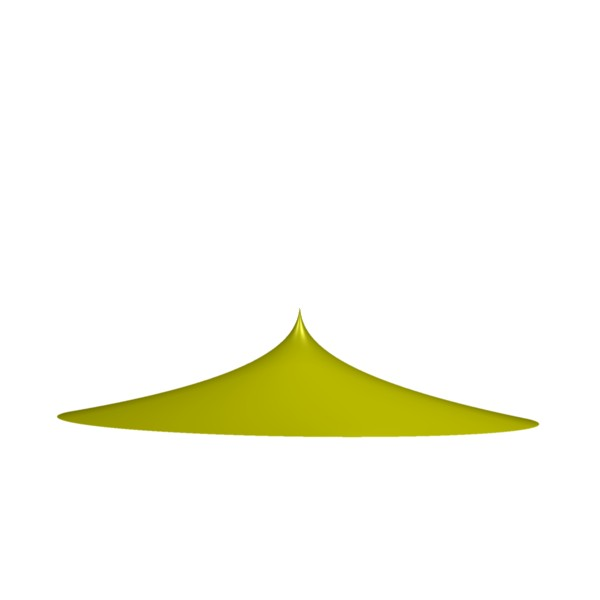
\includegraphics[width=1.2cm]{../../common/images/A4pp_0}
        \end{tabular}
        &
        \begin{tabular}{@{}c@{}}
          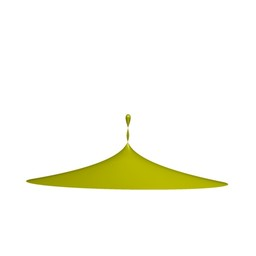
\includegraphics[width=1.2cm]{../../common/images/A4pp_1}
        \end{tabular}
        &
        \begin{tabular}{@{}c@{}}
          
\includegraphics[width=1.2cm]{../../common/images/A4pp_2}
        \end{tabular}
      \end{tabular}
    \end{center}
%    }
      \vspace*{-0.2cm}
      This is realized by the equation: 
    \[x^2(x+a^2)^2(x-a^2)+y^2+z^2.\]
 
\end{surferPage}

